\chapter{Introduction}{``Software engineering today is a race between
  programmers striving to build bigger and better idiot-proof
  programs, and the Universe striving to build bigger and better
  idiots. So far, the Universe is winning.''}{Rich Cook}

As computers become smaller, faster and more reliable, they are
finding uses which could not have been imagined a few decades ago. The
computer was originally conceived and constructed as an equation
solver. This is evidenced by the work carried out by Alan Turing
following construction of---and via the use of---the \emph{bombes} at
Bletchley Park during WWII~\cite{codebook}. This was where the
precursors to the modern-day digital computer were used to decipher
messages coded by the German Enigma Machine. Over the years computers
have grown smaller and more pervasive compared to those found at
Bletchley Park. The reasons for their omnipresence are myriad; they
are cheaper, faster, and easier to use than before. Society itself has
become more and more technologically demanding so that
``computerization'' is seen as an enabler to producing better
products, e.g., cars with anti-lock braking systems, washing machines
and ovens with automatic timers and programmable functions, not to
mention cell phones and wrist watches that have more computing power
than was used to send Man to the Moon. In fact, according to different
industry estimates, of the \emph{six billion} microprocessors produced
annually, 90$\sim$98\% are used in embedded systems and are thus
invisible. The currently perceived major uses of computers include,
but are not limited to:\\

\begin{itemize}
\item{Database management;}
\item{Scientific computation;}
\item{Finance, such as personal accounting all the way to corporate
  finance;}
\item{Office applications such as word processing, spreadsheets and
  presentations;}
\item{Communication via the use of emails, instant messaging and
  social networking;}
\item{Publishing of newspapers and books;}
\item{Entertainment such as movies, video games etc.}
\end{itemize}

\section{Real-time systems}
One of the major uses of computer systems in the past four decades has
been in the domain of \emph{real-time systems}. Contrary to popular
misconception, real-time does not necessarily mean fast; it instead
implies a computation framework where the validity of the results
computed are dependent not only upon the value obtained, but also upon
the time at which they are available. Major applications of real-time
systems include:

\begin{description}
\item[Industrial process control and monitoring:]{Industrial setups
  such as production assembly lines, chemical plants etc. are
  currently controlled and monitored via computer systems. The tasks
  which carry out the control and monitor functions have strict
  temporal constraints to ensure that physical actions are taken at
  the proper time and that the status information displayed is current;}
\item[Vehicle and platform control:]{Modern aircraft are controlled
  via computer systems, called fly-by-wire~\cite{langer@rtsep92}. The
  computer takes information from environmental sensors as well as
  operator input to determine the correct position of the flight
  control surfaces to keep the aircraft stable. Similar systems exist
  for contemporary cars, called drive-by-wire systems. Robot control
  and medical appliances are also real-time systems;}
\item[Vehicle status monitoring and sensor systems:]{Systems such as GPS
  receivers, mission control computers for aircraft as well as certain
  sensors such as radar and sonar are also real-time systems;}
\item[Multimedia:]{Video players need to display a certain amount of
  frames per second and also need to synchronize the audio with the
  video being displayed, this introduces mild temporal constraints and
  thus results in a real-time system.}
\end{description}

Real-time systems fall into one of two main categories from a
point-of-view of validity of results compared to
time~\cite{jensen@ccej97}. Validity in this context means a result
that will ensure that the system conforms to its requirements, and an
invalid result will cause the system to breach its requirements. Hard
real-time systems are those where results obtained after a certain
time (known as the deadline) are completely invalid. As shown in
Fig.~\ref{fig:hard_vs_soft}, the validity of results in a hard
real-time system becomes rapidly invalid after the deadline has
passed; examples of such systems are vehicle control, weapons release,
plant control and robotics systems. On the other hand, values of
results in a soft real-time system become invalid in a more gradual
manner (think of it as an inverse exponential); multimedia systems
fall under this category since a missed deadline may only introduce a
bit of jitter. This dichotomy is needed because in certain
systems, missing a deadline can be catastrophic; whereas in other
systems, a deadline missed may at worst be a nuisance. The two classes
of real-time systems and representative applications that fall in each
or both are shown in Fig.~\ref{fig:rt_apps_overview}.

Computer-controlled real-time systems took off after the seminal paper
of Leyland and Liu on the scheduling of hard real-time
tasks~\cite{liu@jacm73}. This paper introduced the Rate Monotonic
Assignment of priorities for fixed-priority preemptive schedulers, as
well as the Rate Monotonic Analysis technique to determine whether all
tasks will meet their deadlines. Before the advent of this paper and
the techniques it introduced, real-time systems were constructed in an
ad-hoc manner using cyclic executives~\cite{audsley@rts95,
  laplante@rts95}. However, during the 1970s and 1980s it was realized
that this approach led to systems that were inflexible to change and
difficult to maintain; an overview of cyclic executives is given in
Sec.~\ref{sec:scheduling}, also given is an overview of the other
major type of executives, the so-called ``process based executives''.

\begin{figure}
\centering

\includegraphics{figs/hard_vs_soft}
\caption{Validity of computed results in hard (left) vs. soft (right)
  real-time systems.}
\label{fig:hard_vs_soft}
\end{figure}

\begin{figure}
\centering
\includegraphics[scale=0.75]{figs/rt_apps_overview}
\caption{Dichotomy of real-time systems into ``soft'' and
  ``hard''.}
\label{fig:rt_apps_overview}
\end{figure}

The dichotomy provided in Figs.~\ref{fig:rt_apps_overview} and listed
above needs characterization. Some real-time applications need only a
high resolution timer with guaranteed delivery to implement
correctly. An example of this would be a washing machine with multiple
cycles, each of which must run for a certain amount of time. The
micro-controller software in this case would arm the timer with the
correct timeout at the start of each cycle, and would end the cycle on
arrival of the timeout. Similarly, medical devices such as radiation
therapy machines are also examples of real-time systems that require
mainly a high resolution timer in order to know when to stop
emitting. However, since a radiation therapy machine is a critical
piece of equipment, its software must be assured of delivery of said
timer in a fault-tolerant way. Some kind of a heartbeat being sent by
the machine's main software to a fail-safe that will turn the machine
off in case of an emergency is also required. The Therac-25 radiation
therapy machine has been the cause of serious accidents because of a
real-time software bug~\cite{leveson@computer93}.

Another class of real-time systems, as presented in
Fig.~\ref{fig:rt_apps_overview}, are control systems. Real-time
control systems are used to control vehicular platforms. This class of
systems mostly consist of a set of periodic threads---those that are
launched periodically at certain points in time and carry out similar
computations every time---that read data from sensors, compute the
required response and send commands to actuators based on those
calculated responses. This type of system is inherently robust to
missed samples, if a data exchange between various threads does not
take place in one job of the destination thread, then the next job
will probably read the next value and keep the platform reasonably
stable.

The final type of real-time systems are those that are a mix of hard
real-time periodic threads and \emph{sporadic} threads---those that
are launched as a result of the reception of an event---that
communicate amongst themselves to achieve an objective. Examples of
such systems are mission control computers on aircraft, radar systems,
assembly lines etc. Because there are sporadic threads in the
system---e.g., a thread that can be triggered to release a
weapon---therefore in this class of systems, delivery of events must
be assured because a missed event may mean jeopardizing the
functionality of the system.

\section{High-integrity software \& certification}
As stated, because of the fact that modern vehicular platforms are
increasingly sophisticated, there is a growing propensity to control
and monitor them via computers. Within this dichotomy (of control and
monitor functionality), systems for vehicular control have been
computerized due to two main reasons:

\begin{description}
\item[Reduction of labor:]{Systems such as cruise
  control~\cite{jones@jpam90} and autopilots reduce repetitive and
  tedious workload on vehicle operators by taking over higher level
  control functions and automating them according to parameters
  selected by the operator (speed in cruise control and airspeed,
  heading and waypoints in autopilots);}
\item[Managing platform instability:]{Systems such as
  fly-by-wire~\cite{langer@rtsep92} in aircraft and anti-lock braking
  in cars are examples of situations where a human operator
  \emph{cannot} perform the functions required. Modern military
  aircraft have airframes that have relaxed static stability or
  dynamic instability to increase manoeuvrability.  However, such an
  airframe necessitates micro-adjustments of the control surfaces at a
  very high frequency to keep the platform stable, the only solution
  is to introduce a computer into the control loop, which gives rise
  to the fly-by-wire software. Anti-lock braking systems continuously
  check to determine and regulate braking to give optimum non-skid
  behavior, resulting in the shortest possible braking distances.}
\end{description}

Monitoring systems have been computerized simply because a computer is
much more flexible and is capable of providing a much clearer and more
synthesized picture of the state of a system than an analog
solution. Due to this computerization of systems such as aircraft,
cars and trains, a software failure can result in loss of human life,
from whence the term ``high-integrity'' originates. High-integrity
software/systems denote those where a failure would have catastrophic
consequences such as loss of life (in the case of an aircraft or car)
or the loss of a mission (in the case of satellites, probes and other
autonomous systems). Due to the increased impact of software failures
in such systems, governmental agencies usually regulate the software
that can be deployed onboard such platforms.

In the case of aircraft software, the controlling bodies (FAA and
EUROCAE) have developed a standard for the development of avionics
software called ``Software Considerations in Airborne Systems and
Equipment Certification''~\cite{do178b}, usually designated
DO-178B. This standard stipulates requirements on the various phases
of the Software Development Life Cycle (SDLC) that is used for the
development of avionics software; the kind of documentation that must
be done in each phase, the methods of code testing and reports on
those tests that must be carried out, the requirements of traceability
between the various phases of the SDLC, etc. The standard divides
onboard software into one of five \emph{criticality levels}, from A to
E, with Level A software considered the most critical and Level E
software least critical to the correct functioning of the
aircraft. The various criticality levels and the impact of a failure
in software of that criticality level are presented in
Table~\ref{tab:criticality_levels}.

\begin{table}
\centering
\begin{tabular}{|l|l|l|}
\hline
\textbf{Software level}&\textbf{Failure condition}&\textbf{Outcome}\\
\hline
Level A & Catastrophic & Death or injury\\
Level B & Hazardous/Severe-major & Injury\\
Level C & Major & Unsafe workload\\
Level D & Minor & Increased workload\\
Level E & No effect & None\\
\hline
\end{tabular}
\caption{DO-178B Safety Criticality Levels.}
\label{tab:criticality_levels}
\end{table}

The DO-178B standard thus becomes more stringent going from Level E to
Level A software. All fly-by-wire and other control systems must be
Level A software and certified accordingly. Certification normally
occurs via a regulatory body which audits all the artifacts produced
during the development of software; documentation such as requirement
specifications, functional specifications, design, code, test cases
and their results. This is an extremely expensive exercise but one
which remains necessary.

One consequence of the criticality level of a software component is in
the amount and nature of test cases that must be carried out to
achieve the desired confidence in its correctness. For Level B and
below, Decision Testing Coverage (DC) is considered sufficient. DC
implies having at least one test case which can result in a true and a
false evaluation of \emph{every} decision in the code. For a decision
such as \texttt{if(a < 5)}, there would be at least two test cases for
DC testing, one where $a < 5$ and another where $a > 5$. For Level A
components, Modified Condition/Decision Coverage (MC/DC) testing is
stipulated. MC/DC coverage stipulates that there be at least one test
case for each \emph{condition} of every decision such that the
condition be true and one where it be false. For a decision such as
\texttt{if(a < 5 \&\& b > 10)}, MC/DC code coverage would stipulate at
least four test cases, one each with $a < 5$, $a \ge 5$, $b \le 10$
and $b > 10$. Clearly, such test cases can neither be identified nor
generated via hand, and thus instrumented compilers are used which not
only produce the code for a software component, but also the test
cases required to certify it~\cite{gasperoni@ae02}.

The standard also stipulates that the entire software stack deployed
be certified. The operating system (if any), the communication
modules, the device drivers for hardware such as sensors and actuators
must all be certified to the criticality level of the application
software making use of them. Automatic code generators such as Matlab
\simu and SCADE Suite (see Chapter~\ref{chap:biblio})
must also be certified to the criticality level of the software
component they are used to build for the generated code to be exempted
from the certification process.

\section{Model Driven Engineering \& code generation}
Model Driven Engineering (MDE), Model Driven Development (MDD) and its
other aliases are names given to approaches of software and systems
development where~\cite{france@fose07}:

\begin{quote}
\emph{``models are the primary artifacts of development and developers
  rely on computer-based technologies to transform models to running
  systems''}
\end{quote}

A model is an approximation of a system, it serves to enable analysis
of the actual system at a higher level of abstraction, where the
artifacts are much closer to the problem domain than those of the
actual physical system. A typical example of a model are the
mathematical equations of motion that describe the flight of a
projectile fired from the Earths' surface at an angle, resulting in
parabolic motion. The equations provide an approximation of the
physical system in a mathematical domain.

The major push towards MDD approaches began during the 1990s with the
formation of the Object Management
Group\footnote{\url{http://www.omg.org}} and its subsequent
standardization of the Unified Modeling Language or
UML~\cite{uml-super}. However, model driven engineering existed in the
software field before that, approaches such as
OMT~\cite{bruegge@oopsla92}, OOSE~\cite{jacobson-oose} and the Booch
Method~\cite{white-booch}, which are object oriented modeling and
design methods, predate UML by many years. Before that there were
design techniques such as Jackson Structured
Design~\cite{jackson-jsd}. In general, models in computing serve one
or more of three purposes:

\begin{description}
\item[Documentation:]{Because models are more abstract than code and
  are thus nearer the problem domain, they are used and useful for
  documenting the software development process. An example of this
  type of model might be use case diagrams;}
\item[Analysis:]{Being more abstract than code, models are also used
  for carrying out analysis on the system. Examples of these kinds of
  models include Statecharts in UML, which can be used to simulate the
  behavior of systems; the B design method~\cite{abrial@vdm91,
    sorensen-B}, proof engines such as PVS~\cite{owre@cav96} and
  process algebraic techniques such as LOTOS~\cite{garavel@cav07}
  allow proof or verification of system models described in a
  mathematical domain;}
\item[Code generation:]{The final purpose of models in computing is to
  enable automatic generation of code. This automatic code generation
  is an attractive prospect because it can reduce a lot of programming
  effort by supplying a large amount of ``boiler plate'' code.}
\end{description}

The development cycle in a typical MDE based approach---as espoused by
the OMG and typically using UML---is shown in
Fig.~\ref{fig:mde_chain}. After requirements capture has been
completed, a preliminary design is constructed. This design is then
refined or transformed into successively more detailed designs. This
refinement/transformation of a model to another model may be by hand
or automatic. At each refinement of the model, any of a number of
analysis techniques may be applied to it. When the model is detailed
enough, code corresponding to it can be automatically generated. This
code is then modified, and the modifications in code are---in an ideal
world---propagated back up to the model itself, this is called
\emph{roundtrip engineering}. The entire model+code may also be
simulated, in order to study its behavior and perform model level
debugging. Finally, when the model, its generated code \emph{and} the
manual modifications and additions to that code are considered
satisfactory, it can be considered production code and is ready to be
deployed.

\begin{figure}
\centering
\includegraphics[scale=1.0]{figs/mde_chain}
\caption{The steps of a typical MDE development process.}
\label{fig:mde_chain}
\end{figure}

Consider the case of a class diagram, one of the basic notation
methods of object oriented design, where the class hierarchy and
relational structure of a system is given in a graphic format. In UML,
a class is represented by a rectangle with three compartments, for the
name of the class, the member variables and the member functions. The
first design, which is sometimes called the Platform Independent
Model~\cite{mda-guide} or PIM is not dependent upon the programming
language or execution environment that will be eventually chosen. Once
these platform decisions have been made, the PIM can be transformed
automatically to a Platform Specific Model or PSM, which includes
refinements in the model to accommodate the platform's abilities. The
PSM can finally be used to generate code. Fig.~\ref{fig:class} shows a
model artifact for a circle. The PIM is on the left, and the class
\texttt{Circle} contains the attributes to store its position and
radius, and one public member function that calculates its area and
returns it. The PIM to PSM transformation, in this case for C++,
results in the class shown in the middle. Member functions have been
generated to get and set the values of the member variables (newly
generated model elements are shown in bold). This PSM can finally be
used to generate code, as shown in the final part of the figure. The
member functions to access the protected variables are generated
automatically, whereas the function to calculate area must be written
by hand. Thus, the PIM is at the conceptual level of the problem,
whereas the PSM contains more implementation information and is nearer
to the solution space.

As even this trivial example serves to show, MDE can be a powerful
tool in the development of complex software systems and can introduce
major savings of effort, cost and time. The MDE approach stipulates
that models be first class citizens of the development process, not
just afterthoughts added at the end of the lifecycle to satisfy
documentation or contractual requirements. In such a process, models
become as important as the final code, since they actually represent
the code, only at a higher level of abstraction. And even though the
MDE approach is quite new for the more traditional software
development community, it has been successfully used by the real-time
and specifically the aerospace software community for a while now, via
approaches such as HRT-HOOD~\cite{burns@rts94} and
MetaH~\cite{metah-manual}.

\begin{figure}
\centering

\includegraphics{figs/class}
\caption{A class to model a circle, and its transformations to source
  code.}
\label{fig:class}
\end{figure}

\section{Context of the research work}
This section provides an overview of the problem statement that leads
to the research work carried out during this thesis, namely, the
generation of hard real-time system source code from a high-level
architecture description language that is simple, domain specific and
non-ambiguous. It presents, furthermore, the motivation for that work,
and why it is advantageous to undertake such an endeavor.

\subsection{Problem statement}
Given this state of affairs, i.e., the complexity of real-time
software and the strict requirements of safety and quality imposed
upon high-integrity software, it becomes infeasible---if not
impossible---to write such systems purely by hand. Such systems are
now built using one of many high-level languages and tools coupled
with their associated code generators. These high-level languages
allow for a smaller ``vertical distance'' between
requirements/system-level constructs and programming constructs, with
the rest of the vertical distance to be covered done via automatic
code generation from the high-level language. The different types of
high-level languages allow various modeling methodologies and generate
different types of application code, e.g., UML generates an execution
framework and no functional code (in its basic form), which is to run
on a process based executive; \simu and Lustre generate an execution
framework \emph{and} functional code that executes within that
framework on a cyclic executive (see Chapter~\ref{chap:biblio} for an
introduction to these methodologies).

Architecture description languages (ADL) such as Rapide, Wright and
UniCon~\cite{clements@iwssd96} provide a higher level view of the
system and software architecture. They show the various components
that interact together to create a functioning system, the interfaces
of those components and the interconnections between those
interfaces. In a purist ADL approach, the design of the internals of
each component would not be visible, it would be considered a black
box with a certain interface and properties. The internal design of a
component, such as the objects and relations between those objects
that together serve to build up a component, would be the domain of
the modeling language used to design said component (e.g., UML). Since
ADLs have a formal or at least semi-formal semantics and are usually
domain specific, they have historically been an attractive alternative
to the design of real-time---and more specifically
avionics---systems. Examples of ADLs that have been used in such
systems include the HRT-HOOD~\cite{burns@rts94} from the European
Space Agency and MetaH~\cite{metah-manual} from Honeywell (see
Chapter~\ref{chap:biblio} for an introduction to these ADLs).

All of the above-mentioned techniques use a \emph{model
  transformation}, where the source model is transformed into
programming language code which can be compiled and executed. Be it
UML in which the designer models the component using object oriented
methods, or \simu or Lustre where the source model is in the form of
system design blocks and the data flows between them, or even ADLs,
where the source model is in the form of constructs such as processes,
connectors and components; the principal remains the same. By
definition, such design tools and code generators exist for specific
tuples of source modeling language and target programming language.

There exists a need for an architecture description language that is
geared towards hard real-time systems, as opposed to a generic ADL or
modeling language. The reason for this is that the domain is very
specific and the language chosen should be an ideal mix of
expressiveness and simplicity. Expressiveness to allow for the
description of the large class of systems in the domain and simplicity
in order to allow a clear semantics to enable precise, unambiguous
transformations to code. Furthermore, the programming language for
which code should be generated, and the generated code itself, should
be robust, safe and predictable. Of course, once this pair has been
identified, code generation rules for the transformation from
architecture to source code need to be established, and a code
generator itself has to be implemented, as a proof-of-concept in the
first step and eventually an industrial tool as a second step.

The advantages to this approach include, among others, the fact that
an automatic vertical transformation from a system model to code will
intrinsically preserve properties, such as schedulability, the absence
of deadlocks, the integrity of interfaces (since they will be
generated automatically). This allows construction of systems on which
analysis can be carried out on the design rather than on the code
itself and providing systems that are correct by construction (with
respect to the analyses carried out). Thus the problem statement can
be summarized as follows:

\begin{description}
\item[Architecture design language:]{Identification of an architecture
  and modeling language amenable to the design of real-time
  systems. The language chosen must be concise, targeted to the
  domain, semantically non-ambiguous or neutral and agnostic as to the
  target programming language and environment of execution, i.e.,
  whether the target environment is a process based operating system,
  a cyclic executive etc.;}
\item[Programming language and environment:]{Identification of a
  programming language and execution environment that allows for
  robust, deterministic execution;}
\item[Code generator:]{The implementation of a proof-of-concept code
  generator from the architecture language to the programming
  language, which validates the fundamental soundness of the approach,
  as well as the choice of both source architecture language and the
  target programming language and execution environment;}
\item[Case study:]{A significant case study to validate the
  \emph{applicability to the domain} of the approach.}
\end{description}

\subsection{Motivation and objectives of work}
The previous section has detailed \emph{what} needs to be
done. \emph{Why} it needs to be done is detailed here. According to
industry sources, DO-178B certification can add up to 50\% to 100\% to
the cost of software development for newcomers; whereas experienced
suppliers consider that it adds only 20\% to the base cost of
software~\cite{do178b-cost}. In view of this, the European Commission
started the ASSERT Integrated Project (IST-FP6-004033) which brought
together 30 academic and industrial partners, the objective being to
devise new methodologies, techniques and tooling for aerospace
software development. The axes of innovation recognized within the
ASSERT Project were the model driven software engineering approaches
for the development of real-time high-integrity software, the
application of proofs and/or verification to the systems thus
generated and the study of their suitability for and impact upon the
certification process as prescribed by the DO-178B standard.

Towards the achievement of these goals, a number of technologies and
approaches were selected for exploration. One approach selected was
the generation of code from an architecture description language, the
code being generated to conform to the non-functional requirements as
set out in the architecture, i.e., temporal requirements,
communication constructs, and skeleton code generation etc. The
architecture description language selected was the---at the
time---nascent Architecture Analysis \& Design Language~\cite{AS5506}
being developed by the Society of Automotive Engineers in conjunction
with the US Army and major defence contractors. The programming
language chosen was the Ravenscar Profile for High-integrity Systems,
which is a subset of the Ada 95 and Ada 2005 programming languages,
specifically tailored for high-integrity real-time systems. The
execution platform chosen was the Open Ravenscar Kernel
(ORK)~\cite{puente@ae00}, a real-time kernel specifically tailored to
executing programs written with the Ravenscar restrictions. Other axes
to be explored included the use of specialized versions of the Unified
Modeling Language (UML) for the generation of code, the use of formal
models such as Lustre and other synchronous languages to generate
functional code and finally methods of providing automatic or
semi-automatic transformation from requirements to source code,
including proofs of correctness.

Thus, the motivation for this research is to provide a
proof-of-concept that validates the choices made in the context of
this axis of the project, and to prove that a model driven approach
using a modern ADL targeted to the real-time domain coupled with a
programming language and runtime that is robust and geared to the same
class of systems is a feasible and attractive option. In addition,
there is the added objective of presenting a methodology and tooling
to develop not just real-time information systems, but real-time
\emph{control} systems using a process based executive, as opposed to
a cyclic one, which is the current standard practice. This would
allow, in the future, the creation of flexible control systems that
can coexist with other real-time tasks on the same processor. The
objective of the work being, simply, to answer the questions posed in
the problem statement, and to show that the resulting methodologies
and tools in fact \emph{do} reduce the cost and time needed to develop
on board software and that such an approach \emph{can} help in
improving the quality of the software developed and in the
certification needed to deploy it.

\section{Overview of the work presented}
The work presented falls under the objectives outlined in the previous
section. The major contributions carried out were the definition of
code generation rules from the architecture description language
chosen---the AADL---towards Ada, as well as the development of a code
generator to implement and validate these rules. The code generated is
in the form of an \emph{execution framework}. It contains all of the
software entities necessary to ensure correct execution of the system
from the temporal perspective, i.e., threads are generated as they are
defined in the AADL model, with their properties preserved across
transformation from model to code (whether they are sporadic/periodic,
their period or inter-arrival time, the size of their stacks
etc.). Also generated are all the communication and synchronization
entities needed for the threads to work together. This comprises the
message queues between threads as well as any mechanisms to launch
sporadic threads through the sending of events. This means that the
non-functional system requirements specifications can be met via this
generated code; these include the timing requirements and the
communication and synchronization requirements among threads. This
``skeleton'' of the application then needs to be fleshed out with the
functional code of each thread. In more specific terms, the callbacks
of each thread need to be written by hand to meet the functional
specification of the system requirements specification. The code
generated conforms to the Ravenscar Profile for High-integrity
systems~\cite{burns@adalett04}, which is a profile (subset) of the Ada
95 and Ada 2005 languages specifically geared to the high-integrity
real-time domain. Adherence to this profile allows the guarantee of
certain safety properties as well as the ability to perform offline
schedulability analysis of the system.

Furthermore, a specific problem that arises with any asynchronous
real-time system---one that uses a process based executive as opposed
to a cyclic one---is that of the inherent non-determinism in the
dispatching of threads. This non-determinism engenders an impact on
the communication among the different threads, which adversely impact
real-time control systems, and is one of the reasons cyclic executives
are almost exclusively used for such systems. A method of generating
deterministic communication buffers between threads is also developed
and presented. The AADL language is extended to allow the
representation of such connectors and it is explained how these
connectors are integrated into the code generator to enable their
automatic generation in Ada. In addition, since the work done was in
the context of the avionics domain, the correctness of these
connectors is shown via a verification language called
LOTOS~\cite{garavel@cav07}. The code generator developed is augmented
to automatically generate LOTOS code in addition to the Ada
code. Model checking is used on the generated LOTOS code to verify
that the deterministic communication properties of the generated
connectors hold in \emph{all} possible permutations of the schedule of
threads. This kind of verification is very useful for the avionics
domain because of the stringent safety and certification requirements
imposed by the DO-178B standard~\cite{do178b}.

A formal semantics for the generated Ada code is provided as
well. This takes the form of structured operational semantics, or SOS,
as introduced by Plotkin in~\cite{plotkin-sos}. This semantics shows
the evolution of the generated system over time and allows the
formalization of its behavior, leading to---in the future---the
possibility of mathematical treatment of the generated system to
determine and verify various properties upon it.

The final contribution is a large case study carried out with the
tooling developed. It is essentially a reengineering of an existing
Mission Control Computer for a fighter aircraft. The original case
study, called the Generic Avionics Platform, or GAP, was presented
in~\cite{locke@rtss91, locke@irtaw90}. The original GAP case study was
carried out using Ada 83 and was entirely coded by hand, the
specification for the system is called the Generic Aircraft Software
Specification~\cite{locke@sei90}. This system was redesigned using
AADL, and the resulting model was used as an input for the code
generator, which provided the entire software framework in Ada
Ravenscar for the system. The only part of the system that was coded
by hand was the functional response code for each thread in the
system, thus showing the greatly reduced effort for the development of
such systems using automatic code generators and model transformations
and serving the purpose of a proof-of-concept.

The current chapter has given the introduction to the domain, an
overview of the concepts and terminologies used, a context for the
research work, the motivation for the work carried out as well as an
overview of the scientific contributions to the field. However, the
field of model based code generation is not new, neither is the field
of modeling of real-time systems, an overview of the existing
techniques, technologies, tools and languages for the domains of both
code generation and modeling of real-time systems are presented in
Chapter~\ref{chap:biblio}. Because the AADL language as well as the
Ada Ravenscar Profile play such a central role to the research being
presented, an introduction to both is provided in
Chapter~\ref{chap:aadlrs}. The basic code generation rules from AADL
to Ada Ravenscar as well as the architecture of the code generator
implemented to test and validate those rules are the focus of
Chapter~\ref{chap:code_gen}. Chapter~\ref{chap:adv_code} presents
advanced code generation techniques specific to control systems, i.e.,
the deterministic connectors, as well as presenting the LOTOS
verification code that is generated to aid in their certification. The
formal semantics of the generated code is presented in
Chapter~\ref{chap:formal_sem}. Finally, Chapter~\ref{chap:conclusions}
presents the conclusions, discusses the pros and cons of the work
presented and gives a few directions for future
research. Appendix~\ref{chap:rap} gives the details of the avionics
case study. Appendix~\ref{chap:intro_ada} gives an introduction to the
very rich threading and inter-thread communication constructs provided
by the core Ada 95 and Ada 2005 languages for those who may need a
refresher in the subject.

%%% Local Variables:
%%% mode: latex
%%% mode: flyspell
%%% TeX-master: t
%%% End:
